\documentclass[a4paper,12pt]{report}
\setcounter{secnumdepth}{5}
\setcounter{tocdepth}{3}
\input{/usr/share/LaTeX-ToolKit/template.tex}
\begin{document}
\title{Hyperbolic Functions}
\author{沈威宇}
\date{\temtoday}
\titletocdoc
\renewcommand{\arraystretch}{1.5}
\sct{Hyperbolic Functions (雙曲函數)}
\ssc{Hyperbolic Functions}
\sssc{Exponential definitions and properties}
{\fontsize{8pt}{10pt}\selectfont
\begin{longtable}[c]{|p{0.14\textwidth}|p{0.1\textwidth}|p{0.14\textwidth}|p{0.14\textwidth}|p{0.14\textwidth}|p{0.14\textwidth}|}
\hline
    Function & Symbols & Definition & Domain & Range & Odd or even \\\hline\endhead
    Hyperbolic sine (雙曲正弦) & $\sinh x$ & $\frac{e^{x}-e^{-x}}{2}$ & $\bbR$ & $\bbR$ & odd \\\hline
    Hyperbolic cosine (雙曲餘弦) & $\cosh x$ & $\frac{e^{x}+e^{-x}}{2}$ & $\bbR$ & $(1,\infty)$ & even \\\hline
    Hyperbolic tangent (雙曲正切) & $\tanh x$ & $\frac{\sinh(x)}{\cosh(x)}$ & $\bbR$ & $(-1,1)$ & odd \\\hline
    Hyperbolic cotangent (雙曲餘切) & $\coth x$ & $\frac{\cosh(x)}{\sinh(x)}$ & $\bbR\setminus\{0\}$ & $(-\infty,-1)\cup(1,\infty)$ & odd \\\hline
    Hyperbolic secant (雙曲正割) & $\sech x$ & $\frac{1}{\cosh(x)}$ & $\bbR$ & $(0,1]$ & even \\\hline
    Hyperbolic cosine (雙曲餘弦) & $\cosh x$ & $\frac{1}{\sinh(x)}$ & $\bbR\setminus\{0\}$ & $\bbR\setminus\{0\}$ & odd \\\hline
\end{longtable}
\FB}
\sssc{Complex trigonometric functions definitions}
\[\ba
&\sinh(x)=-i\sin(ix)\\
&\cosh(x)=\cos(ix)\\
&\tanh(x)=-i\tan(ix)\\
&\coth(x)=\cot(ix)\\
&\sech(x)=i\sec(ix)\\
&\csch(x)=\csc(ix)
\ea\]
\sssc{Differential equation definitions}
The hyperbolic sine and cosine are the unique solution $(s, c)$ of
\[c'(x)=s(x),\quad s'(x)=c(x)\]
with the initial conditions $s(0)=0,c(0)=1$.

The hyperbolic tangent is the unique solution $f$ of
\[f'=1-f^2\]
with the initial condition $f(0)=0$.
\sssc{Power notation}
\[\ba
&\sinh^n x\coloneq\begin{cases}\qty(\sinh x)^n,\quad n\geq 0\\\arcsinh x,\quad n=-1\end{cases}\\
&\cosh^n x\coloneq\begin{cases}\qty(\cosh x)^n,\quad n\geq 0\\\arccosh x,\quad n=-1\end{cases}\\
&\tanh^n x\coloneq\begin{cases}\qty(\tanh x)^n,\quad n\geq 0\\\arctanh x,\quad n=-1\end{cases}\\
&\coth^n x\coloneq\begin{cases}\qty(\coth x)^n,\quad n\geq 0\\\arccoth x,\quad n=-1\end{cases}\\
&\sech^n x\coloneq\begin{cases}\qty(\sech x)^n,\quad n\geq 0\\\arcsech x,\quad n=-1\end{cases}\\
&\csch^n x\coloneq\begin{cases}\qty(\csch x)^n,\quad n\geq 0\\\arccsch x,\quad n=-1\end{cases}
\ea\]
\ssc{Inverse hyperbolic function (反雙曲函數)}
\sssc{Definition}
\begin{longtable}[c]{|p{0.16\textwidth}|p{0.16\textwidth}|p{0.16\textwidth}|p{0.16\textwidth}|p{0.16\textwidth}|}
\hline
Function & Symbols & Definition & Domain & Range \\
\hline\endhead
    Inverse hyperbolic sine (反雙曲正弦) & \(y=\arcsinh x=\sinh^{-1}(x)=\operatorname{asinh}(x)=\operatorname{arsinh}(x)\) & \(x=\sinh y\) & \(\bbR\) & \(\bbR\) \\ \hline
    Inverse hyperbolic cosine (反雙曲餘弦) & \(y=\arccosh x=\cosh^{-1}(x)=\operatorname{acosh}(x)=\operatorname{arcosh}(x)\) & \(x=\cosh y\) & \([1,\infty)\) & \([0,\infty)\) \\ \hline
    Inverse hyperbolic tangent (反雙曲正切) & \(y=\arctanh x=\tanh^{-1}(x)=\operatorname{atanh}(x)=\operatorname{artanh}(x)\) & \(x=\tanh y\) & \((-1,1)\) & $\bbR$ \\ \hline
    Inverse hyperbolic cotagent (反雙曲餘切) & \(y=\arccoth x=\coth^{-1}(x)=\operatorname{acoth}(x)=\operatorname{arcoth}(x)\) & \(x=\coth y\) & \((-\infty,-1)\cup(1,\infty)\) & \(\bbR\setminus\{0\}\) \\ \hline
    Inverse hyperbolic secant (反雙曲正割) & \(y=\arcsech x=\sech^{-1}(x)=\operatorname{asech}(x)=\operatorname{arsech}(x)\) & \(x=\sech y\) & \((0,1]\) & $[0,\infty)$ \\ \hline
    Inverse hyperbolic cosecant (反雙曲餘割) & \(y=\arccsch x=\csch^{-1}(x)=\operatorname{acsch}(x)=\operatorname{arcsch}(x)\) & \(x=\csch y\) & \(\bbR\setminus\{0\}\) & \(\bbR\setminus\{0\}\) \\ \hline
\end{longtable}
\FB
\sssc{Logarithmatic forms}
\bma
\operatorname{arcsinh} &= \ln\left(x+\sqrt{x^2+1}\right)\\
\operatorname{arccosh} &= \ln\left(x+\sqrt{x^{2}-1}\right),\quad x\geq 1\\
\operatorname{arctanh} &= \frac{1}{2}\ln\left(\frac{1+x}{1-x}\right),\quad\abs{x}<1\\
\operatorname{arccoth} &= \frac{1}{2}\ln\left(\frac{x+1}{x-1}\right),\quad\abs{x}>1\\
\operatorname{arcsech} &= \ln\left(\frac{1}{x}+\frac{\sqrt{1-x^2}}{x}\right),\quad 0<x\leq 1\\
\operatorname{arccsch} &= \ln\left(\frac{1}{x}+\frac{\sqrt{1+x^2}}{\abs{x}}\right),\quad x\neq 0
\eam
\sssc{Hyperbolic functions of inverse hyperbolic functions}
\begin{longtable}[c]{|m{0.1\textwidth}|m{0.12\textwidth}|m{0.12\textwidth}|m{0.12\textwidth}|m{0.12\textwidth}|m{0.12\textwidth}|m{0.12\textwidth}|}
\hline
    \theta & \sinh\theta & \cosh\theta & \tanh\theta & \coth\theta & \sech\theta & \csch\theta \\\hline\endhead
    \arcsinh(x) & x & \sqrt{1+x^2} & \frac{x}{\sqrt{1+x^2}} & \frac{\sqrt{1+x^2}}{x},\quad x\neq 0 & \frac{1}{\sqrt{1+x^2}} & \frac{1}{x},\quad x\neq 0 \\\hline
    \arccosh(x) & \sqrt{x^2-1} & x & \frac{\sqrt{x^2-1}}{x} & \frac{x}{\sqrt{x^2-1}} & \frac{1}{x} & \frac{1}{\sqrt{x^2-1}} \\\hline
    \arctanh(x) & \frac{x}{\sqrt{1-x^2}} & \frac{1}{\sqrt{1-x^2}} & x & \frac{1}{x},\quad x\neq 0 & \sqrt{1-x^2} & \frac{\sqrt{1-x^2}}{x},\quad x\neq 0 \\\hline
    \arccoth(x) & \frac{1}{\sqrt{x^2-1}} & \frac{|x|}{\sqrt{x^2-1}} & \frac{1}{x} & x & \frac{\sqrt{x^2-1}}{|x|} & \sqrt{x^2-1} \\\hline
    \arcsech(x) & \frac{\sqrt{1-x^2}}{x} &{{{ \frac{1}{x} & \sqrt{x^2-1}\operatorname{sgn}\qty(x) & \frac{\operatorname{sgn}\qty(x)}{\sqrt{x^2-1}},\quad|x|>1 & x & \frac{|x|}{\sqrt{x^2-1}} \\\hline
    \arccsc(x) & \frac{1}{x} & \frac{\sqrt{x^2-1}}{|x|} & \frac{\operatorname{sgn}\qty(x)}{\sqrt{x^2-1}},\quad|x|>1 & \sqrt{x^2-1}\operatorname{sgn}\qty(x) & \frac{|x|}{\sqrt{x^2-1}} & x \\\hline
\end{longtable}\FB
\ssc{Identities}
\sssc{雙曲函數基本關係}
\begin{center}
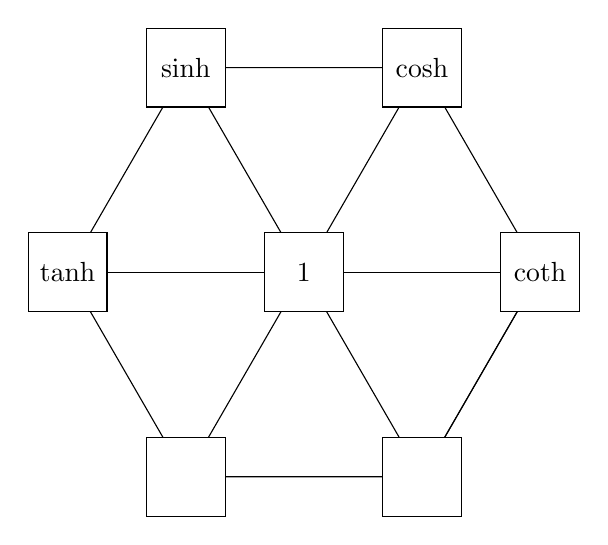
\begin{tikzpicture}
  \foreach \a in {0,60,...,300}
    \node (P\a) at (\a:3) {};
  \draw (P0) -- (P60) -- (P120) -- (P180) -- (P240) -- (P300) -- (P0) -- cycle;
  \draw (P0) -- (P180);
  \draw (P60) -- (P240);
  \draw (P120) -- (P300);
  \draw (P0) -- (P300);
  \node[draw, fill=white, minimum size=1cm, anchor=center] at (P0) {$\coth$};
  \node[draw, fill=white, minimum size=1cm, anchor=center] at (P60) {$\cosh$};
  \node[draw, fill=white, minimum size=1cm, anchor=center] at (P120) {$\sinh$};
  \node[draw, fill=white, minimum size=1cm, anchor=center] at (P180) {$\tanh$};
  \node[draw, fill=white, minimum size=1cm, anchor=center] at (P240) {$\sech$};
  \node[draw, fill=white, minimum size=1cm, anchor=center] at (P300) {$\csch$};
  \node[draw, fill=white, minimum size=1cm, anchor=center] at (0,0) {$1$};
\end{tikzpicture}
\end{center}
\bit
\item 名稱:左側三者為正;右側三者為餘;上面二者為弦;中間二者為切;下面二者為割。
\item 倒數關係:三條通過中心點的線,其兩端者互為倒數,相乘為1。
\item 商數關係:六邊形周上,連續三個頂點形成的連線,其兩端者相乘等於中間者。
\item 平方(Pythagorean)關係:圖中有三個倒正三角形,其在右上頂點者之平方減去在左上頂點者之平方等於在下方頂點者之平方。
\eit
\sssc{歐拉關係}
\[\ba&\cosh x+\sinh x=e^x\\
&\cosh x-\sinh x=e^{-x}\ea\]
\sssc{正切萬能公式}
\[\ba
&\sinh\theta=\frac{2\tanh\frac{\theta}{2}}{1-\tanh^2\frac{\theta}{2}}\\
&\cosh\theta=\frac{1+\tanh^2\frac{\theta}{2}}{1-\tanh^2\frac{\theta}{2}}\\
&\tanh\theta=\frac{2\tanh\frac{\theta}{2}}{1+\tanh^2\frac{\theta}{2}}
\ea\]
\sssc{二倍角公式}
\[\ba
\sinh 2\theta&=2\sinh\theta\cosh\theta\\
\cosh 2\theta &=1+2\sinh^2\theta\\
&=2\cosh^2\theta-1\\
&=\cos^2\theta-\sin^2\theta
\ea\]
\sssc{半角公式或平方化倍角公式}
\[\ba
\sinh\frac{\theta}{2}  &=\operatorname{sgn}(x)\sqrt{\frac{\cosh\theta-1}{2}}\\
\cosh\frac{\theta}{2}  &=\sqrt{\frac{\cosh\theta+1}{2}}\\
\tanh\frac{\theta}{2}  &=\operatorname{sgn}(x)\sqrt{\frac{\cosh\theta-1}{\cosh\theta+1}}\\
&=\frac{\sin\theta}{\cos\theta+1}\\
&=\frac{\cos\theta-1}{\sin\theta}\\
&=\frac{\sin\theta+\cos\theta-1}{\sin\theta+\cos\theta+1}\\
&=\coth\theta-\csch\theta
\ea\]
\sssc{三倍角公式}
\[\sinh 3\theta=3\sinh\theta+4\sinh^3\theta\]
\[\cosh 3\theta=4\cosh^3\theta-3\cosh\theta\]
\[\tanh 3\theta=\frac{3\tanh\theta+\tanh^3\theta}{1+3\tan^2\theta}\]
\sssc{和差角公式}
\[\sinh\qty(\alpha +\beta)=\sinh\alpha\cosh\beta +\cosh\alpha\sinh\beta\]
\[\sinh\qty(\alpha -\beta)=\sinh\alpha\cosh\beta -\cosh\alpha\sinh\beta\]
\[\cosh\qty(\alpha +\beta)=\cosh\alpha\cosh\beta +\sinh\alpha\sinh\beta\]
\[\cosh\qty(\alpha -\beta)=\cosh\alpha\cosh\beta -\sinh\alpha\sinh\beta\]
\[\tanh\qty(\alpha +\beta)=\frac{\tanh\alpha+\tanh\beta}{1+\tanh\alpha\tanh\beta}\]
\[\tanh\qty(\alpha -\beta)=\frac{\tanh\alpha-\tanh\beta}{1-\tanh\alpha\tanh\beta}\]
\[\coth\qty(\alpha +\beta)=\frac{\coth\alpha\coth\beta +1}{\coth\alpha +\coth\beta}\]
\[\coth\qty(\alpha -\beta)=\frac{\coth\alpha\coth\beta -1}{\coth\beta -\coth\alpha}\]
\[\sech\qty(\alpha +\beta)=\frac{\sech\alpha\sech\beta}{1+\tanh\alpha\tanh\beta}=\frac{\csch\alpha\csch\beta}{\coth\alpha\coth\beta+1}\]
\[\sech\qty(\alpha -\beta)=\frac{\sech\alpha\sech\beta}{1-\tanh\alpha\tanh\beta}=\frac{\csch\alpha\csch\beta}{\coth\alpha\coth\beta-1}\]
\[\csch\qty(\alpha +\beta)=\frac{\csch\alpha\csch\beta}{\coth\alpha+\coth\beta}=\frac{\sech\alpha\sech\beta}{\tanh\alpha+\tanh\beta}\]
\[\csch\qty(\alpha -\beta)=\frac{\csch\alpha\csch\beta}{\coth\beta-\cot\alpha}=\frac{\sech\alpha\sech\beta}{\tanh\alpha-\tanh\beta}\]
\sssc{平方化雙曲正切平方公式}
\[\sinh^2\theta=\frac{\tanh^2\theta}{1-\tanh^2\theta}\]
\[\cosh^2\theta=\frac{1}{1-\tan^2\theta}\]
\[\coth^2\theta=\frac{1}{\tan^2\theta}\]
\[\sech^2\theta=1-\tanh^2\theta\]
\[\csch^2\theta=\frac{1-\tan^2\theta}{\tan^2\theta}\]
\sssc{和差化積公式}
\bma
\sinh\alpha +\sinh\beta &= 2\sinh\frac{\alpha +\beta}{2}\cosh\frac{\alpha -\beta}{2}\\
\sinh\alpha -\sinh\beta &= 2\cosh\frac{\alpha +\beta}{2}\sinh\frac{\alpha -\beta}{2}\\
\cosh\alpha +\cosh\beta &= 2\cosh\frac{\alpha +\beta}{2}\cosh\frac{\alpha -\beta}{2}\\
\cosh\alpha -\cosh\beta &= 2\sinh\frac{\alpha +\beta}{2}\sinh\frac{\alpha -\beta}{2}
\eam
\sssc{積化和差公式}
\bma
2\sin\alpha\cos\beta &= \sin (\alpha +\beta)+\sin (\alpha -\beta)\\
2\cos\alpha\sin\beta &= \sin (\alpha +\beta)-\sin (\alpha -\beta)\\
2\cos\alpha\cos\beta &= \cos (\alpha +\beta)+\cos (\alpha -\beta)\\
2\sin\alpha\sin\beta &= \cos (\alpha +\beta)+\cos (\alpha -\beta)
\eam
\end{document}

